The channel steering vector is given by
\begin{equation*}
    e_r\left(\Omega\right) = \frac{1}{\sqrt{N_r}} \begin{pmatrix}
    1 \
    e^{-j 2 \pi \Delta_r \Omega} \
    e^{-j 2 \pi \Delta_r 2\Omega} \
    \vdots \
    e^{-j 2 \pi \Delta_r (N_r - 1)\Omega}
    \end{pmatrix}.
\end{equation*}
where $\Delta_r$ is the normalized array spacing, and $\Omega = \cos \phi$ represents the direction cosine, which is related to the incidence angle. In this assignment, $\Delta_r$ is set to $\frac{1}{2}$, which is the optimal spacing, and the incidence angles are randomly generated as $\phi \in \left[-\pi/2, \pi/2\right]$. The steering vectors are shown below:

\begin{figure}[H]
    \centering
    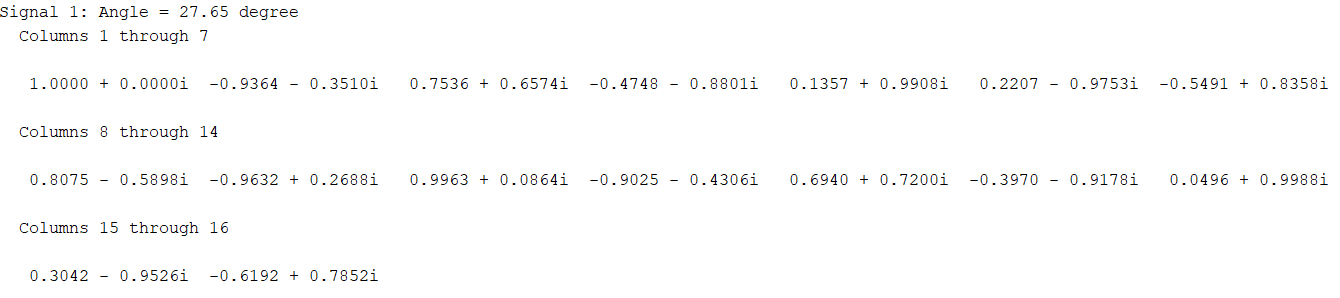
\includegraphics[scale = 0.6]{s1.png}
\end{figure}
\begin{figure}[H]
    \centering
    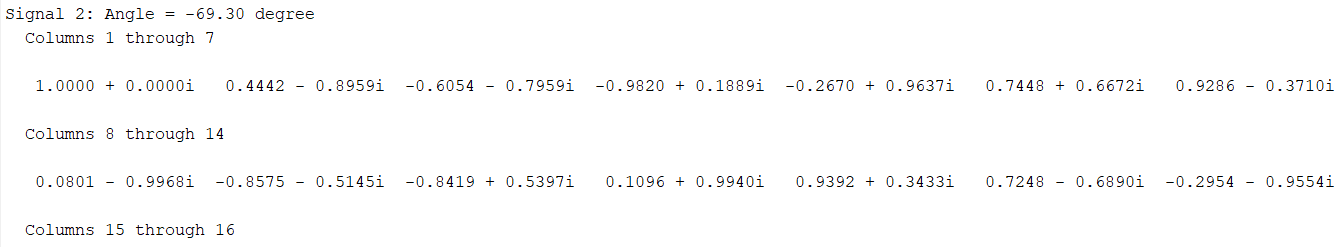
\includegraphics[scale = 0.6]{s2.png}
\end{figure}
\begin{figure}[H]
    \centering
    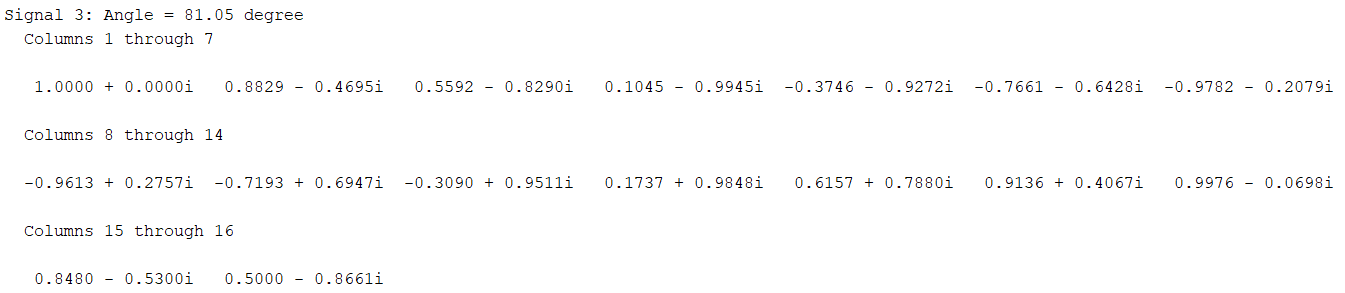
\includegraphics[scale = 0.6]{s3.png}
\end{figure}
\begin{figure}[H]
    \centering
    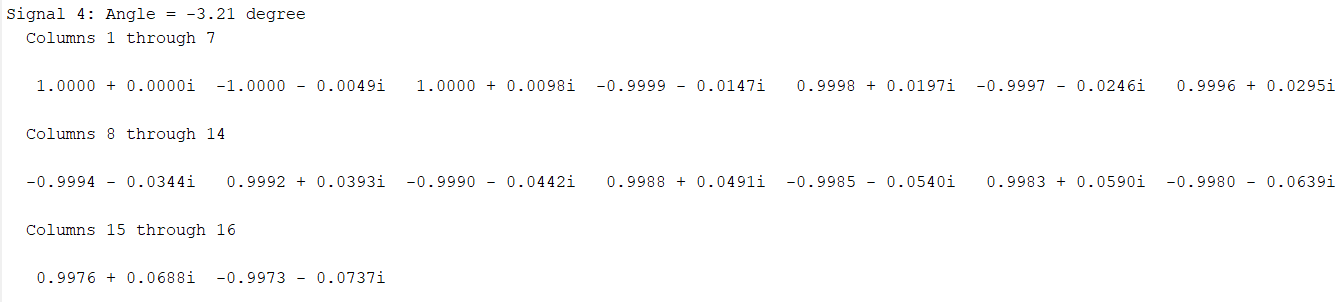
\includegraphics[scale = 0.6]{s4.png}
\end{figure}
\begin{figure}[H]
    \centering
    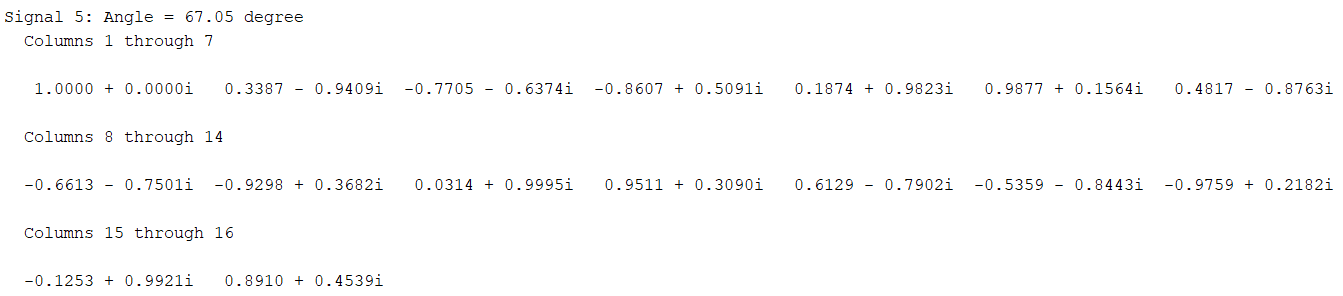
\includegraphics[scale = 0.6]{s5.png}
\end{figure}